% Options for packages loaded elsewhere
\PassOptionsToPackage{unicode}{hyperref}
\PassOptionsToPackage{hyphens}{url}
\PassOptionsToPackage{dvipsnames,svgnames,x11names}{xcolor}
%
\documentclass[
  letterpaper,
  DIV=11,
  numbers=noendperiod]{scrartcl}

\usepackage{amsmath,amssymb}
\usepackage{iftex}
\ifPDFTeX
  \usepackage[T1]{fontenc}
  \usepackage[utf8]{inputenc}
  \usepackage{textcomp} % provide euro and other symbols
\else % if luatex or xetex
  \usepackage{unicode-math}
  \defaultfontfeatures{Scale=MatchLowercase}
  \defaultfontfeatures[\rmfamily]{Ligatures=TeX,Scale=1}
\fi
\usepackage{lmodern}
\ifPDFTeX\else  
    % xetex/luatex font selection
\fi
% Use upquote if available, for straight quotes in verbatim environments
\IfFileExists{upquote.sty}{\usepackage{upquote}}{}
\IfFileExists{microtype.sty}{% use microtype if available
  \usepackage[]{microtype}
  \UseMicrotypeSet[protrusion]{basicmath} % disable protrusion for tt fonts
}{}
\makeatletter
\@ifundefined{KOMAClassName}{% if non-KOMA class
  \IfFileExists{parskip.sty}{%
    \usepackage{parskip}
  }{% else
    \setlength{\parindent}{0pt}
    \setlength{\parskip}{6pt plus 2pt minus 1pt}}
}{% if KOMA class
  \KOMAoptions{parskip=half}}
\makeatother
\usepackage{xcolor}
\setlength{\emergencystretch}{3em} % prevent overfull lines
\setcounter{secnumdepth}{-\maxdimen} % remove section numbering
% Make \paragraph and \subparagraph free-standing
\ifx\paragraph\undefined\else
  \let\oldparagraph\paragraph
  \renewcommand{\paragraph}[1]{\oldparagraph{#1}\mbox{}}
\fi
\ifx\subparagraph\undefined\else
  \let\oldsubparagraph\subparagraph
  \renewcommand{\subparagraph}[1]{\oldsubparagraph{#1}\mbox{}}
\fi


\providecommand{\tightlist}{%
  \setlength{\itemsep}{0pt}\setlength{\parskip}{0pt}}\usepackage{longtable,booktabs,array}
\usepackage{calc} % for calculating minipage widths
% Correct order of tables after \paragraph or \subparagraph
\usepackage{etoolbox}
\makeatletter
\patchcmd\longtable{\par}{\if@noskipsec\mbox{}\fi\par}{}{}
\makeatother
% Allow footnotes in longtable head/foot
\IfFileExists{footnotehyper.sty}{\usepackage{footnotehyper}}{\usepackage{footnote}}
\makesavenoteenv{longtable}
\usepackage{graphicx}
\makeatletter
\def\maxwidth{\ifdim\Gin@nat@width>\linewidth\linewidth\else\Gin@nat@width\fi}
\def\maxheight{\ifdim\Gin@nat@height>\textheight\textheight\else\Gin@nat@height\fi}
\makeatother
% Scale images if necessary, so that they will not overflow the page
% margins by default, and it is still possible to overwrite the defaults
% using explicit options in \includegraphics[width, height, ...]{}
\setkeys{Gin}{width=\maxwidth,height=\maxheight,keepaspectratio}
% Set default figure placement to htbp
\makeatletter
\def\fps@figure{htbp}
\makeatother

\usepackage{booktabs}
\usepackage{longtable}
\usepackage{array}
\usepackage{multirow}
\usepackage{wrapfig}
\usepackage{float}
\usepackage{colortbl}
\usepackage{pdflscape}
\usepackage{tabu}
\usepackage{threeparttable}
\usepackage{threeparttablex}
\usepackage[normalem]{ulem}
\usepackage{makecell}
\usepackage{xcolor}
\KOMAoption{captions}{tableheading}
\usepackage{float}
\floatplacement{table}{H}
\makeatletter
\@ifpackageloaded{caption}{}{\usepackage{caption}}
\AtBeginDocument{%
\ifdefined\contentsname
  \renewcommand*\contentsname{Table of contents}
\else
  \newcommand\contentsname{Table of contents}
\fi
\ifdefined\listfigurename
  \renewcommand*\listfigurename{List of Figures}
\else
  \newcommand\listfigurename{List of Figures}
\fi
\ifdefined\listtablename
  \renewcommand*\listtablename{List of Tables}
\else
  \newcommand\listtablename{List of Tables}
\fi
\ifdefined\figurename
  \renewcommand*\figurename{Figure}
\else
  \newcommand\figurename{Figure}
\fi
\ifdefined\tablename
  \renewcommand*\tablename{Table}
\else
  \newcommand\tablename{Table}
\fi
}
\@ifpackageloaded{float}{}{\usepackage{float}}
\floatstyle{ruled}
\@ifundefined{c@chapter}{\newfloat{codelisting}{h}{lop}}{\newfloat{codelisting}{h}{lop}[chapter]}
\floatname{codelisting}{Listing}
\newcommand*\listoflistings{\listof{codelisting}{List of Listings}}
\makeatother
\makeatletter
\makeatother
\makeatletter
\@ifpackageloaded{caption}{}{\usepackage{caption}}
\@ifpackageloaded{subcaption}{}{\usepackage{subcaption}}
\makeatother
\ifLuaTeX
  \usepackage{selnolig}  % disable illegal ligatures
\fi
\usepackage{bookmark}

\IfFileExists{xurl.sty}{\usepackage{xurl}}{} % add URL line breaks if available
\urlstyle{same} % disable monospaced font for URLs
\hypersetup{
  pdftitle={Homework 1},
  pdfauthor={Sammy Ramacher},
  colorlinks=true,
  linkcolor={blue},
  filecolor={Maroon},
  citecolor={Blue},
  urlcolor={Blue},
  pdfcreator={LaTeX via pandoc}}

\title{Homework 1}
\usepackage{etoolbox}
\makeatletter
\providecommand{\subtitle}[1]{% add subtitle to \maketitle
  \apptocmd{\@title}{\par {\large #1 \par}}{}{}
}
\makeatother
\subtitle{Research Methods, Spring 2024}
\author{Sammy Ramacher}
\date{}

\begin{document}
\maketitle

My answers to the homework questions are described below. Note that I do
the analysis for these answers in a separate \texttt{R} script. You can
read in the full data as part of your markdown file, but that takes some
time to compile to pdf. So I run the analysis separately, save the
workspace with only the summary stats, figures, and tables that I need,
and then load the workspace in the final qmd. My analysis file is
available in the analysis folder. Enjoy!

\newpage

\section{Enrollment Data}\label{enrollment-data}

Answer the following based on the enrollment data:

\vspace{.2in}

\noindent 1. How many observations exist in your current dataset?

First we need to create the enrollment data. Working with the Medicare
Advantage Github Repository, you should have created a ``full.ma.data''
object. Then we just count the total number of plans. This yields
13,276,162 total observations in the full dataset, which means there are
13,276,162 unique combinations of contract/plan/county/year.

\newpage

\noindent 2. How many different \emph{plan\_types} exist in the data?

To do this, we need to group by plan type and count the number of unique
plan types. I did this by creating a table of unique plan types (since
we'll need this for the next question anyway). The resulting table
yields 18 rows, so there are 18 total plan types.

\newpage

\noindent 3. Provide a table of the count of plans under each plan type
in each year.

See Table~\ref{tbl-plans}.

\begin{verbatim}
Warning in styling_latex_scale(out, table_info, "down"): Longtable cannot be
resized.
\end{verbatim}

\begin{longtable}[t]{lrrrrrr}

\caption{\label{tbl-plans}Plan types by year}

\tabularnewline

\toprule
Plan Type & 2010 & 2011 & 2012 & 2013 & 2014 & 2015\\
\midrule
Medicare Prescription Drug Plan & 893,609 & 771,694 & 815,223 & 826,907 & 1,122,209 & 991,457\\
HMO/HMOPOS & 506,802 & 528,473 & 507,272 & 530,909 & 523,304 & 479,275\\
Local PPO & 417,551 & 515,700 & 636,701 & 633,884 & 664,716 & 704,993\\
PFFS & 385,733 & 45,781 & 36,423 & 31,919 & 24,905 & 13,658\\
Employer/Union Only Direct Contract PDP & 28,700 & 28,697 & 28,669 & 25,526 & 25,528 & 25,630\\
\addlinespace
Regional PPO & 24,442 & 22,773 & 21,602 & 19,970 & 19,773 & 17,578\\
1876 Cost & 6,035 & 6,851 & 7,633 & 7,731 & 7,069 & 7,157\\
HCPP - 1833 Cost & 3,604 & 11 & 11 & 10 & 9 & 9\\
Employer/Union Only Direct Contract PFFS & 3,332 & 3,329 & 3,323 & 0 & 0 & 0\\
National PACE & 717 & 781 & 858 & 953 & 1,118 & 1,216\\
\addlinespace
Continuing Care Retirement Community & 142 & 0 & 0 & 0 & 0 & 0\\
MSA & 135 & 6,421 & 6,416 & 6,431 & 6,449 & 6,518\\
PSO (State License) & 123 & 176 & 171 & 0 & 0 & 0\\
ESRD I & 117 & 0 & 0 & 0 & 0 & 0\\
Pilot & 53 & 3 & 3 & 2 & 2 & 2\\
\addlinespace
ESRD II & 8 & 0 & 0 & 0 & 0 & 0\\
Medicare-Medicaid Plan HMO/HMOPOS & 0 & 0 & 0 & 265 & 1,319 & 4,130\\
\bottomrule

\end{longtable}

\newpage

\noindent 4. Remove all special needs plans (SNP), employer group plans
(eghp), and all ``800-series'' plans. Provide an updated table after
making these exclusions.

I remove the relevant plans just by applying the relevant filter to the
full ma data and then creating the table of plan types. Counts of
different plan types with these exclusions are presented in
Table~\ref{tbl-plans2}

\begin{verbatim}
Warning in styling_latex_scale(out, table_info, "down"): Longtable cannot be
resized.
\end{verbatim}

\begin{longtable}[t]{lrrrrrr}

\caption{\label{tbl-plans2}Revised plan types by year}

\tabularnewline

\toprule
Plan Type & 2010 & 2011 & 2012 & 2013 & 2014 & 2015\\
\midrule
Medicare Prescription Drug Plan & 391,205 & 295,458 & 289,044 & 278,091 & 301,082 & 269,153\\
PFFS & 54,119 & 22,038 & 17,449 & 12,945 & 6,053 & 4,232\\
HMO/HMOPOS & 34,460 & 33,931 & 37,551 & 37,179 & 38,893 & 36,588\\
0 & 29,733 & 0 & 0 & 0 & 0 & 0\\
Local PPO & 11,652 & 13,874 & 17,030 & 17,089 & 17,169 & 16,728\\
\addlinespace
Regional PPO & 10,659 & 10,995 & 11,279 & 9,660 & 10,420 & 8,531\\
1876 Cost & 4,923 & 5,829 & 6,647 & 6,759 & 6,207 & 6,329\\
National PACE & 717 & 781 & 858 & 953 & 1,118 & 1,216\\
ESRD I & 117 & 0 & 0 & 0 & 0 & 0\\
PSO (State License) & 97 & 141 & 143 & 0 & 0 & 0\\
\addlinespace
MSA & 68 & 131 & 132 & 145 & 163 & 232\\
Continuing Care Retirement Community & 64 & 0 & 0 & 0 & 0 & 0\\
Medicare-Medicaid Plan HMO/HMOPOS & 0 & 0 & 0 & 265 & 1,319 & 4,130\\
\bottomrule

\end{longtable}

\newpage

\noindent 5. Merge the the contract service area data to the enrollment
data and restrict the data only to contracts that are approved in their
respective counties. Limit your dataset only to plans with non-missing
enrollment data. Provide a graph showing the average number of Medicare
Advantage enrollees per county from 2008 to 2015.

Now we can join that dataset to our MA data. I use an inner join, which
means I'm only taking rows that match in both datasets. I then apply the
filter to remove plans with missing enrollment data, from which we can
form the graph of average enrollments per county, as reflected in
Figure~\ref{fig-enroll}.

\begin{figure}

\centering{

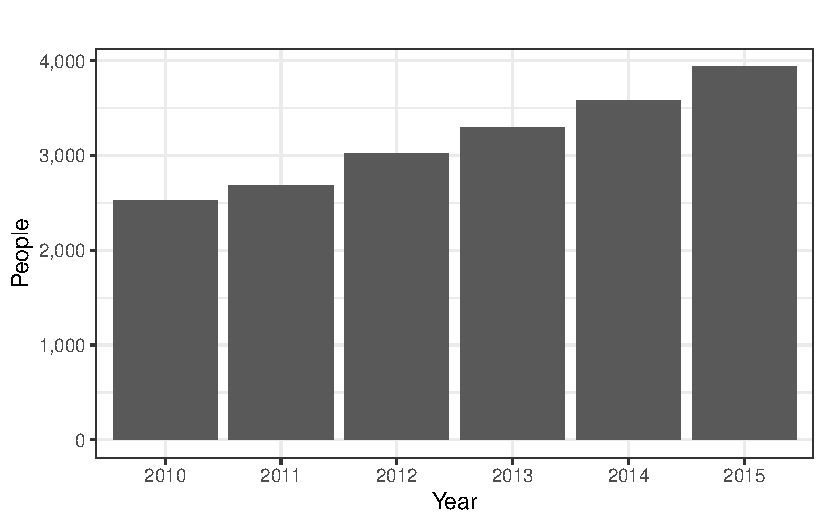
\includegraphics{hwk1-answers_files/figure-pdf/fig-enroll-1.pdf}

}

\caption{\label{fig-enroll}Average Enrollment}

\end{figure}%

\newpage

\section{Premium Data}\label{premium-data}

\noindent 6. Merge the plan characteristics data to the dataset you
created in Step 5 above. Provide a graph showing the average premium
over time. Don't forget about formatting!

As mentioned in the instructions, we first need to merge in the market
penetration data to provide a crosswalk between the plan/contract info
and the plan characteristics. Next we need to fill in the state
information. I do this by creating a table of unique state names and
then merging this back to the original data. Finally, we can read in the
premium data and merge that information to the final dataset

A graph of average premiums over time is presented in
Figure~\ref{fig-premium}. Note the spike in premiums in 2014. What's
that?

\begin{figure}

\centering{

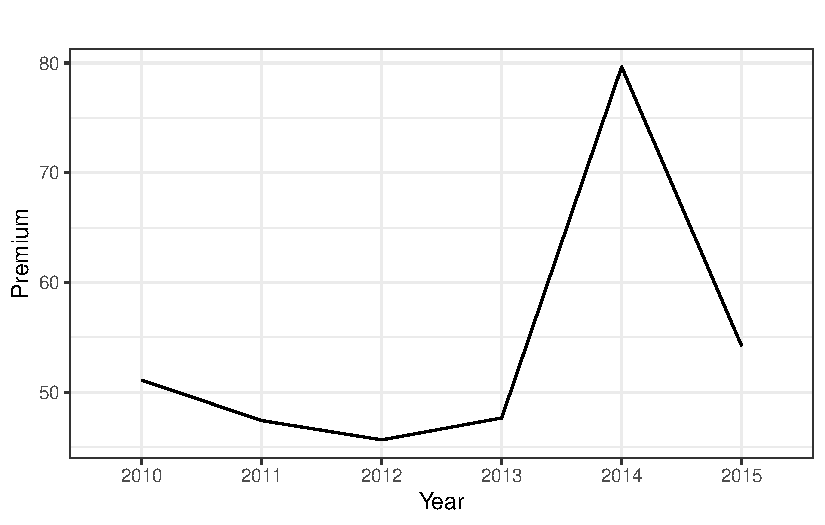
\includegraphics{hwk1-answers_files/figure-pdf/fig-premium-1.pdf}

}

\caption{\label{fig-premium}Average Premiums}

\end{figure}%

\newpage

\noindent 7. Provide a graph showing the percentage of \$0 premium plans
over time. Also\ldots remember to format things.

A graph of the percentage of \$0 premium plans is in
Figure~\ref{fig-zero}. Consistent with Figure~\ref{fig-premium}, we see
a large drop (down to 0\%) in the percentage of 0 premium plans in 2014.
If we also look at the number of missing premium plans, we would see a
big spike in 2014. Effectively, these premiums are 0 in some years but
listed as missing in 2014.

\begin{figure}

\centering{

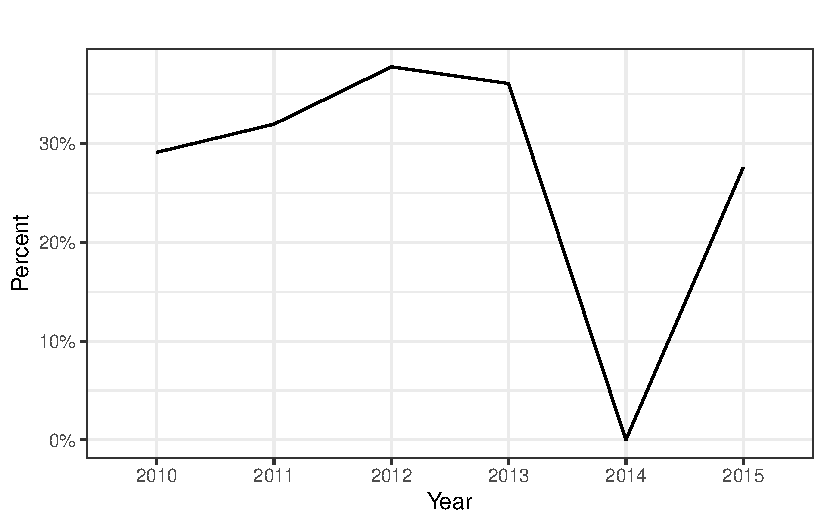
\includegraphics{hwk1-answers_files/figure-pdf/fig-zero-1.pdf}

}

\caption{\label{fig-zero}Share of 0 premium plans}

\end{figure}%

\newpage

\section{Summary Questions}\label{summary-questions}

With all of this data work and these great summaries, let's take a step
back and think about what all this means.

\vspace{.2in}

\noindent 8. Why did we drop the ``800-series'' plans?

These are plans that aren't available to all people. There are sometimes
referred to as ``Employer Group Waiver Plans''. Since not everyone has
access to these plans, summaries including these plans aren't reflective
of an average enrollee's experience in the Medicare Advantage program.

\newpage

\noindent 9. Why do so many plans charge a \$0 premium? What does that
really mean to a beneficiary?

All beneficiaries still pay a Part B premium (nearly \$180 in 2022). So
a plan with no premium really just means it's a plan with no additional
premium in excess of the Part B premium.

\newpage

\noindent 10. Briefly describe your experience working with these data
(just a few sentences). Tell me one thing you learned and one thing that
really aggravated you.

One thing I learned as an instructor is that it takes a couple of days
to get all of the kinks out in the workflow process (git, github, r, vs
code, quarto). I think next year I'll have a 1-2 hour tutorial on a
weekend or something to make sure everyone has this process in place
before we start on the homework. On the bright side, this is the biggest
dataset we'll work with all year!



\end{document}
